
\maketitle

The fundamental idea behind this strategy is to assign each thread to a subset of the workspace. Each thread will manage it's own kd-tree containing all sampled points within it's assigned sub-space. 

\begin{figure}[h]
\begin{centering}
    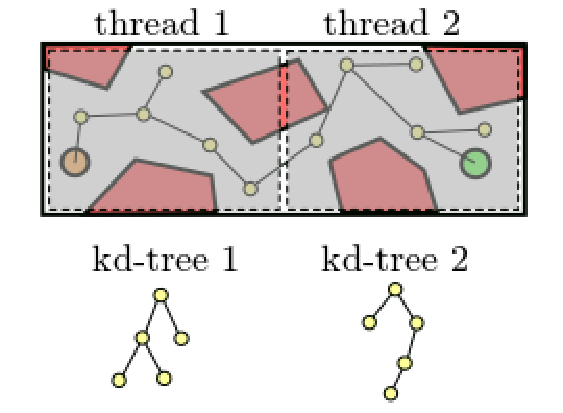
\includegraphics[scale=1]{\figfile{fig/thread_kdtree}}
    \caption{Division Strategy}
\end{centering}
\end{figure}

\section{Sampling}

Sampling should be rather straightforward. Mutsuo Saito and Makoto Matsumoto have realsed CUDA codes for using Merseinne Twister to generate uniform random samples on the GPU. Their webpage for this implementation (MTGP) is at \url{http://www.math.sci.hiroshima-u.ac.jp/~m-mat/MT/MTGP/index.html}

The kernel uses a block of memory to maintain the state of the algorithm, and outputs an array of random numbers to another block of memory. 

\section{Nearest Neighbor}

We can potentially do nearest neighbor search in the same way as a single-thread RRT*, by searching over all nodes for the nearest neighbor. This can be somewhat of a challenge though if each thread has it's own kd tree, because we first need to find the nearest non-empty bin(s), and then find the nearest nodes in those bins. Therefore we may want to super-impose an additional data structure on top of the thread-divisioned kd trees.  

Assuming that the number of threads is unchanging then we can store a quad-tree to index the threads' kd-trees. This will use a constant amount of space and we can further speed up future searches if, at the end of each search, the thread stores the distance from it's bin to the bin where the nearest node was found. Subsequent searches can start from that depth in the kd-tree, up until the thread starts finding nearest nodes in the neighboring bins. Each nearest neighbor search will always have to at least look in it's own bin, and all of its neighboring bins, because nodes near the edge of the bin could be closer to nodes of the neighboring bin than nodes of it's own bin.

\begin{figure}[h]
\begin{centering}
    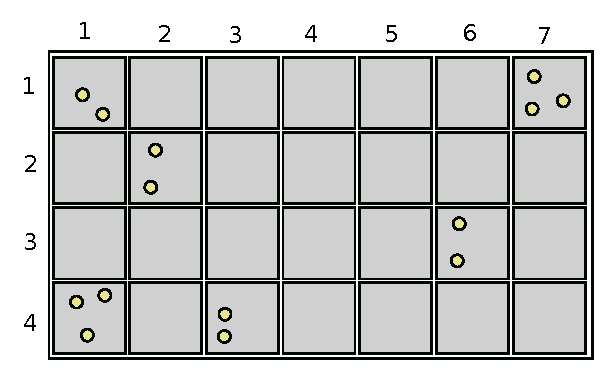
\includegraphics[scale=1]{\figfile{fig/nonempty_search}}
    \caption{Non-empty Search}
    \label{fig:nonempty}
\end{centering}
\end{figure}


We'd like a data structure which will allow us to efficiently find the nearest bin(s) which contain at least one node. We'd like this structure to provide efficient queries for all bins. While it is true that the number of threads will be constant (and thus, searching over all of them will be constant time), there may be thousands of threads and we can potentially see a significant improvement by an added index. 

Consider figure \ref{fig:nonempty}. If we generate a sample in bin (2,4), then we only need to search bins (2,2), (4,3), and (3,6) for the nearest node. If we generate a sample in bin (1,1), we only need to search bins (1,1) and (2,2). In the worst case, we would have to search all the bins on the perimeter of the workspace. 

\subsection{Full Bins}

When all bins contain at least one node, then the nearest node to a sample will be in the bin where the sample was generated, or any of the eight other bins around it. We can assign separate threads to search each of the trees, storing all the results in shared memory, and then running a reduction on it. 

\subsection{Prior to full bins}

\subsubsection{Index Idea}

Here is an idea. For each bin, store an integer corresponding to the unilateral distance (measured in number of bins on the longest edge) to the nearest non-empty bin. For bin (4,4) in figure \ref{fig:nonempty} that distance will be 2. Initially, each bin will store the distance from itself to the farthest edge of the workspace. After each successful nearest node search, it updates that distance by updating the distance to the bin where the nearest node was found. The idea is that the nearest node in all bins outside that radius will be, by definition, further away than the node that was just found. 

\subsubsection{Enumerating non-empty bins}

To enumerate non-empty bins, we can assign one thread per bin within the perimeter defined by the above index. For a given sample, if the stored index is $d$, then this will require at most $d^2$ threads. Each of these threads will simply check whether their bin is non-empty. They store the result of this check in shared memory, and then we perform a reduction to write an array of non-empty bin indices which we should check. The reduction should start at the center, and abort early on the first perimeter containing
 a non-empty bin.


\subsubsection{Quadrants}

Once all bins are occupied by at least one node, we can quickly narrow down the search to only four bins. Consider the following figure.

\begin{figure}[h]
\begin{centering}
    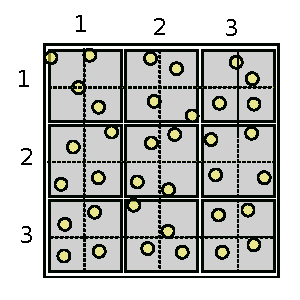
\includegraphics[scale=1]{\figfile{fig/nonempty_full_quad}}
    \caption{Quandrants}
\end{centering} 
\end{figure}

For a sample generated in bin (2,2), in the south-east quadrant, then, assuminb all quadrants of all bins are occupied, the nearest node may be in 

\begin{enumerate}
    \item Any quadrant of bin (2,2)
    \item The northeast quadrant of bin (3,3)
    \item Either of the western quadrants of bin (2,3)
    \item Either of the northern quadrants of bin (3,2)
\end{enumerate}

This is a simple way to narrow down the search, but I'm not sure it will really offer us a gain in runtime. If it does, we can either store four separate kd-trees per bin, or we can add an additional index to the kd-tree which stores the root element of the smallest (hyper-) rectangle (subtree) that fully contains the quadrant.

Nevermind, this is dumb. Rename ``quadrant'' as ``bin'', and all we're advocating here is quadroupling the number of bins.





\section{Steering}

For simple steering functions (i.e. for a single integrator) or for functions which cannot be parallelized, in calculating the path from one node to another, the thread who created the sample will be the one who calculates the trajectory. For functions which may be parallelized (i.e. trajectory optimization) we may actually want to serialize over samples, and parallelize the steering of an individual node pair. 

\section{Collision Checking (Single Paths)}

Collision checking may likewise be done in series or parallel. Series has the benefit of aborting early. Is there a bandwidth benefit to parallel collision checking if serial collision checking can maximize throughput?


\section{Near Nodes}

\section{Rewiring}



\subsection{Child node lists}

How should we store the child node lists? Does the scheduling of the algorithm yield a reasonable (soft) maximum number of child nodes? If it does, can we enforce such a maximum and still guarentee optimality? What do we do if a desired parent is already saturated, do we find another parent, or do we just drop the node?

Will we hit a huge performance penalty if the child node lists are stored as linked lists? Can we marginalize this penalty by creating a linked list where some $n$ successive entries in that list are stored successively in memory?

\begin{figure}[h]
\begin{centering}
    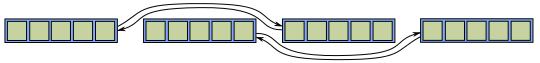
\includegraphics[scale=1]{\figfile{fig/child_list}}
    \caption{Linked-list of arrays}
\end{centering} 
\end{figure}

\subsection{Synchronization}

Reparenting may lead to a race condition in two ways. 

\subsubsection{On the child}
If a particular node is being considered for rewiring, it is possible that two separate threads have generated ``better'' parents for it. We need to serialize the actual reparenting over the different potentials. 

If all potential rewirings in a particular bin are considered by the thread owning that bin, then this is naturally serialized. However, this will require an exchange of data, since the thread who recognizes that the node should be considered (i.e. the thread that does the near node search) may be a different thread.



\subsubsection{On the parent}
If a particular newly-sampled node provides a better path for multiple children, then we need to serialize the storage of the child pointers, as the next available pointer may be written both multiple parents. 

If all potential children are enumerated by the thread who sampled the node, this is naturally serialized.








\end{document}

 